\documentclass{article}
\usepackage{tikz}
\usepackage{graphicx}
\usepackage{float}
\usetikzlibrary{mindmap,positioning}

\begin{document}

\section{Izbira modela}
\subsection{Osrednja arhitektura}
\begin{itemize}
    \item{Pristopi so bili ovrednoteni posamično, s predpostavko medsebojne neodvisnosti (zaradi zahtevnosti treniranja)}
    \item{Modeli vrednoteni relativno med vozlišči na istem nivoju grafa}

    \item{Označbe metod:}
    \begin{itemize}
        \item{Siva - nepreizkušeno}
        \item{Zelena - izbrano za končni model}
        \item{Rdeča - neizbrano/slabše}
        \item{Modra - primerjava ni nujno primerna}
        \item{Rumena - ne predstavlja opazne izboljšave}
    \end{itemize}
\end{itemize}

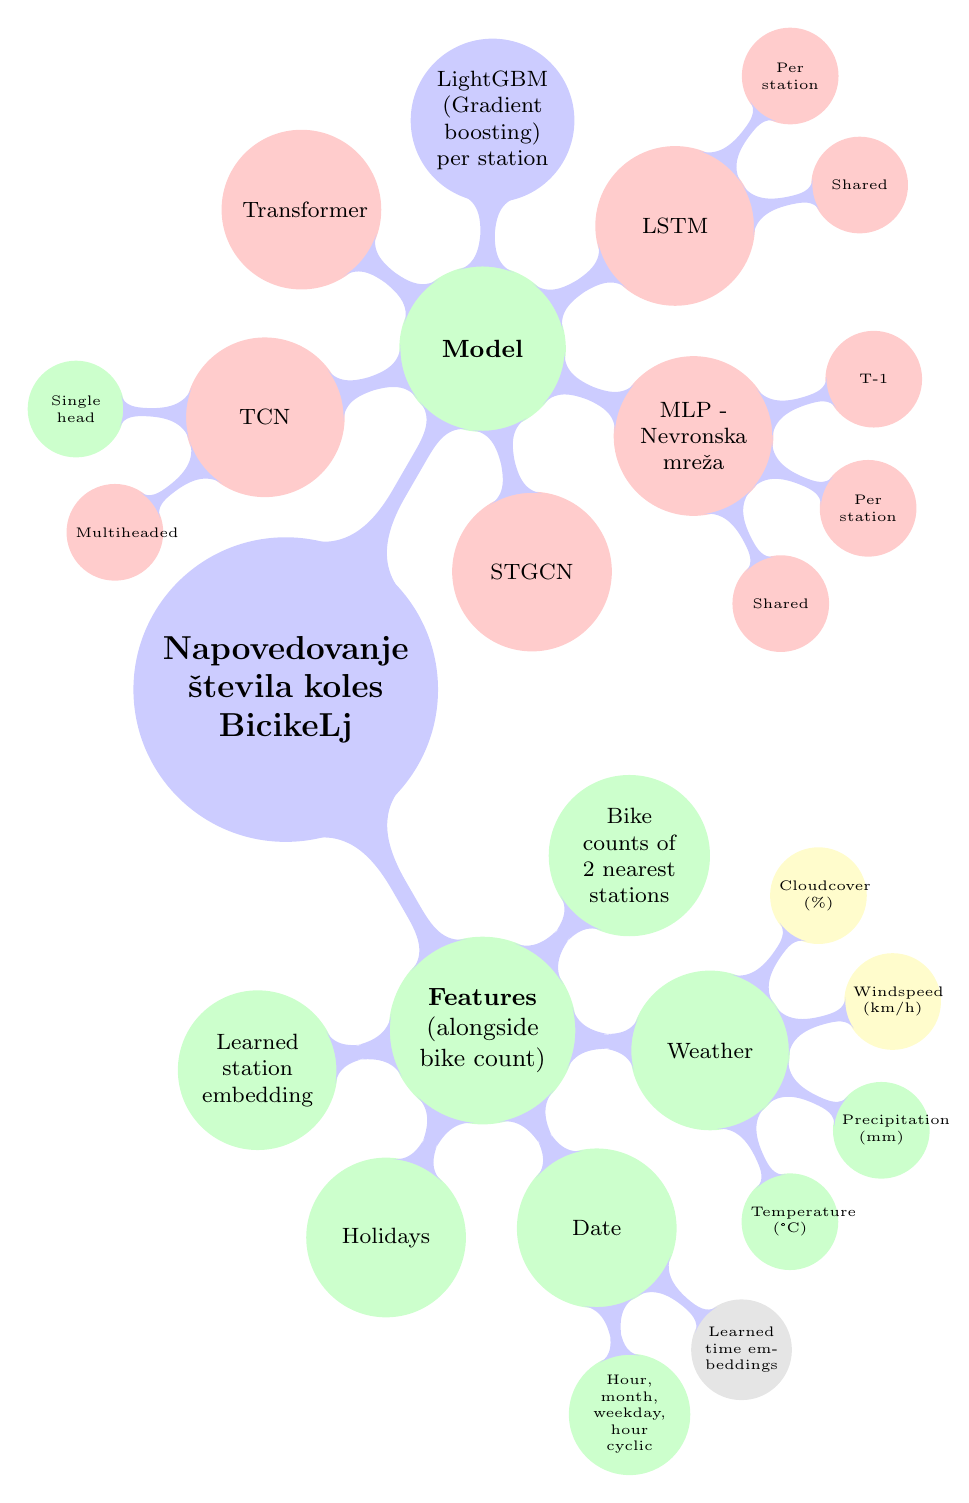
\begin{tikzpicture}[mindmap,
    every node/.style={concept, draw, circle, thick, text=black, minimum size=2cm},
    concept color=blue!20,
    grow cyclic,
    level 1/.append style={sibling angle=120},
    level 2/.append style={sibling angle=55},
    level 3/.append style={sibling angle=40, every node/.append style={minimum size=1.2cm}},
    ]
    \node {\textbf{Napovedovanje števila koles BicikeLj}}
      child { node[concept color=green!20] {\textbf{Features} (alongside bike count)}
          child { node[concept color=green!20] {Learned station embedding} }
          child { node[concept color=green!20] {Holidays} }
          child { node[concept color=green!20] {Date}
              child { node[concept color=green!20] (datetime) {Hour, month, weekday, hour cyclic} }
              child { node[concept color=gray!20] {Learned time embeddings} }
          }
          child { node[concept color=green!20] {Weather}
              child { node[concept color=green!20] {Temperature (°C)} }
              child { node[concept color=green!20] {Precipitation (mm)} }
              child { node[concept color=yellow!20] {Windspeed (km/h)} }
              child { node[concept color=yellow!20] {Cloudcover (\%)} }
          }
          child { node[concept color=green!20] {Bike counts of 2 nearest stations} }
        }
        child { node[concept color=green!20] {\textbf{Model}}
          child { node[concept color=red!20] {STGCN} }
          child { node[concept color=red!20] {MLP - Nevronska mreža} 
              child { node[concept color=red!20] {Shared} }
              child { node[concept color=red!20] {Per station} }
              child { node[concept color=red!20] {T-1} }
          }
          child { node[concept color=red!20] (lstm) {LSTM} 
              child { node[concept color=red!20] {Shared} }
              child { node[concept color=red!20] {Per station} }          
          }
          child { node[concept color=blue!20] {LightGBM (Gradient boosting) per station} }
          child { node[concept color=red!20] {Transformer} }
          child { node[concept color=red!20] {TCN} 
              child { node[concept color=green!20] {Single head} }
              child { node[concept color=red!20] {Multiheaded} }          
          }
        };

\iffalse
\node[draw=none, fill=none, text=black, above left=-15mm and 5mm of knn] {
  \scriptsize
  \begin{itemize}
    \setlength\itemsep{1pt}        % spacing between items
    \setlength\parskip{0pt}        % paragraph spacing
    \setlength\parsep{0pt}         % spacing between item and paragraph
    \item ugotovitev: \\ \textbf{Napoved primitivnega modela je $\approx 36\mathrm{MAE}$}
  \end{itemize}
};
\fi

\end{tikzpicture}

\section{Vrednotenje}
\begin{itemize}
    \item Učna množica je razdeljena na \textbf{train}, \textbf{validation} in \textbf{holdout} podmnožice v razmerju 0.8:0.1:0.1. Primere validation in holdout podmnožice predstavljajo okna 48+4 ur in so iz originalne učne množice izvzeti naključno po času. Med treniranjem je model ovrednoten na validation podmnožici. Uporablja se early stopping glede na MAE na validation množici. Končni model je evalviran na holdout množici. Te tri podmnožice imajo prazen presek.
    \item Iskanje hiperparametrov in primerjava med modeli je bila izvedena relativno na natančnost napovedi na holdout množici (enak seed).
    \item Za tekmovalni strežnik je bil model streniran na \textbf{train} podmnožici, ki je predstavljala 90\% originalne učne množice. Ostalih 10\% je predstavljala \textbf{validation} množica. Holdout množice v tem primeru ni bilo.
\end{itemize}

\subsection{Izbira hiperparametrov}

\begin{table}[h!]
\centering
\begin{tabular}{c|c|c|c|c|c}
\textbf{Combination} & \textbf{hidden\_dim} & \textbf{dropout} & \textbf{lr} & \textbf{weight\_decay} & \textbf{batch\_size} \\
\hline
1 & 64 & 0.2 & 0.001 & 0.0001 & 64 \\
2 & 64 & 0.2 & 0.0005 & 0.0001 & 128 \\
3 & 64 & 0.4 & 0.001 & 0.0001 & 128 \\
4 & 64 & 0.4 & 0.001 & 0.0    & 64 \\
5 & 64 & 0.2 & 0.001 & 0.0001 & 32 \\
\end{tabular}
\caption{Najboljših 5 konfiguracij hiperparametrov.}
\label{tab:top5_configs}
\end{table}

Early stopping patience = 8
\begin{figure}[H]
    \centering
    \includegraphics[width=1.0\textwidth]{imgs/grid_search.png}
    \caption{Primer 5 najboljših kombinacij hiperparametrov}
    \label{fig:grid_search}
\end{figure}


Ostali hiperparametri kot so \textbf{kernel\_size}, \textbf{dilation}, \textbf{n\_layers} (number of temporal blocks) itd. so bili izbrani nesistematično s poskušanjem.

\begin{table}[h!]
\centering
\begin{tabular}{|l|l|l|l|l|}
\hline
\textbf{Batch size} & \textbf{LR} & \textbf{Weight decay} & \textbf{Dropout} & \textbf{Hidden dim} \\
\hline
128 & 5e-4 & 1e-4 & 0.2 & 64 \\
\hline
\end{tabular}
\caption{Izbrani hiperparametri modela}
\label{tab:hyperparams1}
\end{table}
\begin{table}[h!]
\centering
\begin{tabular}{|l|l|l|l|l|}
\hline
\textbf{Kernel size} & \textbf{\#Blocks} & \textbf{Stride} & \textbf{Station embed dim} \\
\hline
3 & 4 & 1 & 8 \\
\hline
\end{tabular}
\caption{Izbrani hiperparametri modela}
\label{tab:hyperparams1}
\end{table}

Model je na holdout množici, ki predstavlja skupaj 160 napovedi za 40 48 urnih sekvenc, dosegel MAE \textbf{9.4291}. Za natančnejšo oceno bi morali enako vrednotenje pognati še večkrat pri razlčnih seed vrednostih, ali pa izvesti prečno preverjanje. Model enake arhitekture streniran za tekmnovalni strežnik, je dosegel MAE \textbf{9.2866}.

Čas treniranja modela je na Nvidia A100 grafičnih karticah vzel približno 1.22s na epoho.

\section{Razlaga modela}
\includegraphics[scale=0.7]{imgs/model.png}
\subsection{SHAP}
\begin{center}
\includegraphics[scale=0.7]{imgs/shap_values.png}
\newpage
\includegraphics[scale=0.5]{imgs/shap_importance.png}
\end{center}

\section{Dodatne slike}
\includegraphics[scale=0.5]{imgs/cross_correlation.png}
\includegraphics[scale=0.6]{imgs/correlation_vs_dist.png}

\end{document}
